\chapter{High-voltage electrical system}
\paragraph{} The design and provision of electrical power systems for aerodrome visual and radio navigation aids will be such that an equipment failure will not leave the pilot with inadequate visual and non-visual guidance or misleading information. Therefore, Electrical system will be designed following the regulations from \cite{ICAO2006}, \cite{Sanidad2009} and \cite{Standards2016}.

	\section{Electrical system general design}
	\paragraph{} For the airport electrical system, two independent incoming power sources, coming from widely separated sections of the electricity network beyond the aerodrome, with each supplying separate substations on the aerodrome property will be used. Selection is, therefore, on the basis of least probability of simultaneous failure of both sources. 
	
	Power to the aerodrome main power substation will be supplied at a high voltage (over 5 000 volts). Then the voltage will be reduced on the aerodrome substation to an intermediate voltage (2 000 to 5 500 volts) for distribution within the aerodrome. A further step-down of voltage will be necessary to match the required input voltage of visual aids equipment.
	
	Aerodrome reliability will be improved by using a double loop system from independent primary sources operating as open rings fed from two transformers at each station.
	
	\begin{figure}[H]
		\centering
		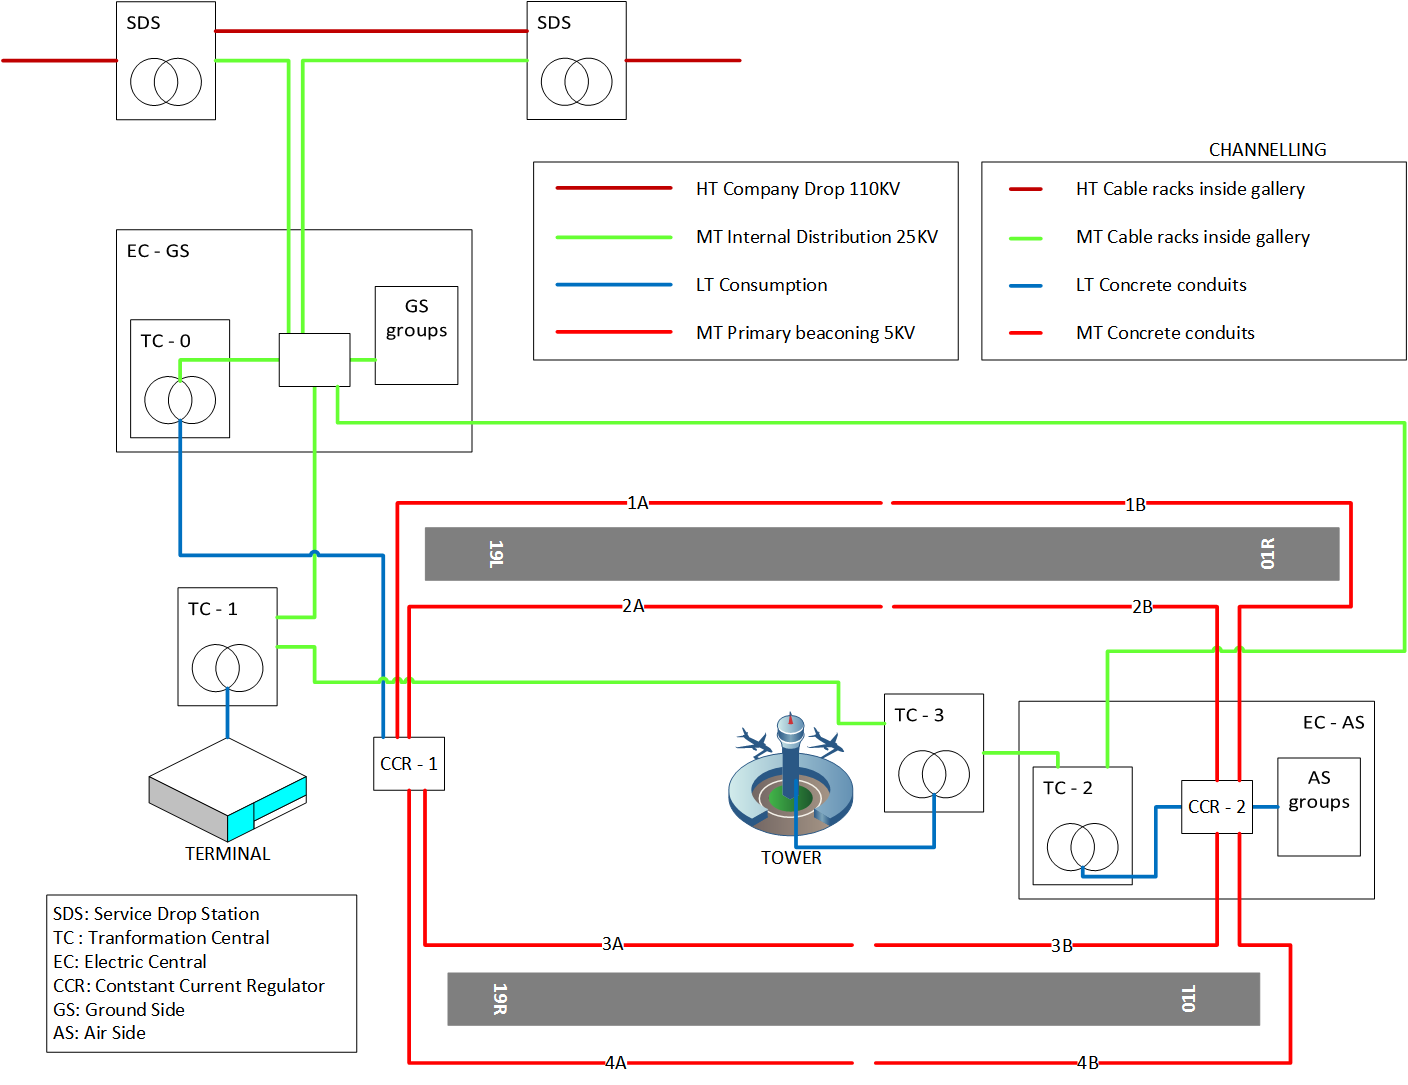
\includegraphics[clip, trim=0cm 0cm 0cm 0cm, width=1.15\textwidth]{./images/electric/esquema_electrico.png}
		\caption{General electric system scheme}
		\label{electricScheme}
	\end{figure}
	
	
	\section{Connection sub-stations}
	
	\section{Electric powerplant}
	
	\section{Electrical transformation center}
	
	\section{Channeling and distribution of the electrical system}
	